\chapter{Introducción}\label{chap:introduccion}

Este capítulo introductorio se abordara los principales conceptos relacionados con el trabajo de tesis, comenzando con una descripción del marco de trabajo de investigación, el objetivo principal, los objetivos secundarios, fundamentos y motivación que nos llevo a realizar la pregunta de investigación; ademas se dará un resumen del estado del arte de la temática en el ámbito espacial describiendo la metodología empleada para el desarrollo de software implementado.  Para finalizar se describe los capítulos posteriores que dan al lector una guía de como esta organizado el trabajo de investigación.


\section{Contexto de la Tesis}\label{sec:contexto}
El presente trabajo se realizó para recibir el grado de \textbf{\textit{Maestría en desarrollos informáticos de aplicación espacial}}. El mismo se encuadra dentro del Plan Nacional Espacial Argentino vigente (2004-2015), a través de \ac{conae} en conjunto con la unidad académica \ac{unlam} y la unidad de desarrollo \ac{sur}.

Esta investigación se centra en aplicar  algoritmos de \textit{Computer Vision}  y \textit{Machine Learning} para la localización y reconocimiento de objetos en una imagen satelital.


\section{Objetivo principal de la tesis}\label{sec:obj_general}

El objetivo principal de este trabajo de tesis es, analizar y utilizar algoritmos para el  reconocimiento de patrones sobre imágenes satelitales de la superficie terrestre haciendo uso de metodologías de visión por computadoras (\ac{cv}, por sus siglas en ingles) y aprendizaje automático (\ac{ml}, por sus siglas en ingles); buscando realizar una prototipo experimental de estas técnicas computacionales.


\subsection{Objetivos específicos }\label{sub:obj_especifico}
A continuación se expondrá los objetivos específicos que permiten en su conjunto establecer los pasos a seguir para  cumplir con el objetivo primario:
\begin{itemize}
 \item Investigar técnicas de \ac{cv} y \ac{ml} aplicadas al reconocimiento de patrones.
 \item Evaluar la factibilidad de ser implementadas sobre imágenes satelitales.
 \item Desarrollar un prototipo de software que permita detectar patrones utilizando diferentes técnicas computacionales de \ac{cv} y \ac{ml}.
 \item Validación de los resultados obtenidos.
\end{itemize}


\section{Fundamentación/Motivación}\label{sec:fundamentacion}

Partiendo del objetivo principal, la presente investigación se centra en evaluar diversas técnicas de \ac{cv} y \ac{ml} aplicadas a imágenes satelitales terrestres.

Las regiones de interés que se aborda en esta tesis son:
\begin{itemize}
	\item Golfo San Matías (Rio Negro-Argentina).
	\item Laguna Mar Chiquita (Córdoba-Argentina).
\end{itemize}

Las imágenes que se utilizaron para el desarrollo fueron obtenidas de los instrumento  \ac{viirs}. Estas imágenes se asemejan a las características de la cámara NIR/SWIR del SABIA-MAR(Satélite Argentino Brasileño para Información del Mar); cuya factibilidad de ser usada en un CubeSat fue evaluada en el marco del proyecto integrador \ac{fs} de \ac{conae}.

El reconocimiento de patrones en imágenes es un área que en la actualidad se incremento con la aparición de nuevas técnicas y de los avances de poder de cómputo. La aplicación de técnicas computacionales tanto de  \ac{cv} y \ac{ml} en reconocimiento de patrones  en tierra y en vuelo, nos permite aprovechar la información contenida en la imagen  automatizando el proceso de extracción de los datos.

Diversas son las ventajas que nos permitirán realizar estos nuevos enfoques computacionales en el área espacial. Los principales beneficios al aplicar técnicas de \ac{cv} y \ac{ml} son: 
\begin{itemize}
\item \textbf{Calibración y apuntamiento}: brindar un mecanismo de apoyo para colaborar con el apuntamiento y la calibración óptica del satélite; mayormente para CubeSat, satélites de menor tamaño, que no poseen un mecanismo eficiente de determinación orbital como un Star-tracker o GPS debido a que son satélites de bajo costo además con relación al tamaño del mismo; con esto se podrá mejorar el apuntamiento detectando las regiones y comparando con los planes de pasadas  establecidos, a la vez dar soporte para poder calibrar la cámara óptica de acuerdo a la región.
\item \textbf{Almacenamiento en memoria}: una de las grandes desventajas que tienen los satélites, es la escasez de recursos en vuelo, teniendo un mecanismo de reconocimiento de patrones se podrá almacenar aquellas imágenes de interés minimizando y optimizando  así el uso de la memoria.
\item \textbf{Exploración del espacio profundo}: ya existe en la actualidad ejemplos de técnicas de reconocimiento aplicadas al análisis de datos en tiempo real, esto es necesario  porque el tiempo de transmisión de información a grandes distancias es alto, es por ello que es necesario poder procesar la información en tiempo real y realizar una predicción automática de los datos obtenidos.
\item \textbf{Predicción de coaliciones:} por medio de \ac{cv} nos permitirá prevenir las posibles coaliciones a causa de la chatarra espacial. 
\item \textbf{Detecciones de catástrofes naturales}: a través de diferentes algoritmos de reconocimiento de patrones en vuelo nos permitirá realizar una alerta temprana en situaciones de desastre detectando por ejemplo focos de incendios, inundaciones, derrames de petroleo, etc.
\item \textbf{Monitoreo del territorio nacional}: evaluando a través de imágenes satelitales las frontera nacional.
\end{itemize}

\section{Estado del Arte} \label{sec:estadodelarte}

En este sección describiremos las diversas investigaciones y trabajos realizados con imágenes satelitales aplicando técnicas de \ac{cv} y \ac{ml} resaltando el estado actual y uso de la temática abordada.

\subsection{Aplicaciones en el ámbito espacial}\label{sub:estadodelacuestion}

Las aplicaciones de \ac{cv} en el ámbito espacial son cada ves mas utilizadas, desde el estudio de un área determinada hasta implementaciones echas a bordo de un satélite artificial. Este avance se dio gracias a diversos factores en el campo de la informática; en primer lugar la creciente capacidad de computo, con procesadores de mayor rendimiento y el auge de las unidades de procesamiento grafico (GPU, por sus siglas en ingles). En segundo lugar la aparición de algoritmos y frameworks mas eficiente en el uso de reconocimiento de patrones, de los que podemos nombrar el uso de redes neuronales convolucionales (\ac{cnn} por sus siglas en ingles), en el capitulo \ref{chap:marcoteorico} se describirá con mas detalle. 

Otro factor que no podemos dejar de nombrar son la aparición de vehículos aéreo no tripulado (UAVs, por sus siglas en ingles), esto permitió utilizar algoritmos de \ac{cv} sobre imágenes de mayor tamaño. La presencia en el mercado de pequeños UAVs de bajo costo con capacidad para portar pequeñas cámaras de vídeo de alta resolución y de realizar despegue vertical con posibilidad de movimiento en cualquier dirección del espacio, hace posible abordar nuevos retos en el campo de la detección y seguimiento de determinadas situaciones de la realidad \citep{Lanillos}.

Actualmente en el campo de reconocimiento de patrones sobre imágenes satelitales se pude ver que la mayoría de los trabajos que se realizaron en el área espacial han sido aplicado en tierra, gran parte de estos trabajos se basan en estudiar las característica del terreno. Estas aplicaciones son cada vez mas explotada no solo por agencias espaciales sino por entidades educativas, publicas y privadas. 

Para empezar vamos a comenzar citando el siguiente trabajo realizado por \citep{Cheang}; en este articulo se describe el uso de técnicas de \ac{ml} usando aprendizaje supervisado. El método para la extracción y clasificación de los datos utilizado se baso en dos enfoques; por un lado se utilizaron técnicas de \textit{sliding window}  \citep{sliding_windows}para la obtención de regiones candidatas desarrollado en el capitulo \ref{chap:marcoteorico}, por otro se aplicaron redes neuronales covolucionales (\ac{cnn}), método muy utilizado para el reconocimiento de objeto en una imagen. Otro ejemplo encontrado en la literatura aplicando  \textit{aprendizaje no supervisado} es para la clasificación del uso de la tierra a partir de imágenes satelitales multi-temporales, en este paper \citep{pnn}, se utilizo imágenes del satélite LANSAT y SPOT usando redes neuronales probabilista, estas técnicas realizan un agrupamiento de datos, \textit{clusters}, y realizan la clasificación creando las fronteras entre los diferentes \textit{clusters} de datos para su posterior reconocimiento.

En el blog titulado \textit{Una imagen vale más que mil palabras}, los autores destacan el beneficio de aplicar procesamiento en imágenes para la toma de decisiones que agregan valor a su negocio. En este articulo describen la posibilidad de conocer el historial de inundaciones de una región rural aplicando técnicas \ac{ml} sobre imágenes satelitales\footnote{Fuente:http://www.7puentes.com/blog/2017/12/11/agtech-imagenes-satelitales-una-imagen-vale-mas-que-mil-palabras/}.

El uso de \ac{cv} permite crear mapas urbanos a partir de imágenes satelitales como menciona en el articulo \citep{detectionHOG}; en el mismo usa \ac{cv} para crear mapas urbanos que determinan cambios temporales en una determinada región geográfica. En este trabajo los autores proponen dos módulos para el desarrollo; por un lado usar \textit{HOG} , histograma de gradientes orientados,\citep{HOG_algoritmo} para la extracción de características en la imagen y patrones binarios locales (LBP, pos sus siglas en ingles)\citep{LBP}, como método descriptor de característica; por ultimo para clasificar los datos utilizaron clasificadores lineales, que se desarrollarán en el capitulo \ref{chap:marcoteorico}. 

\cite{usman} en su articulo describe la extracción de características de una imagen satelital aplicando métodos de  detección de bordes, \textit{edges proposal}\citep{proposal}, descripto en la sección (Sec: \ref{sub:regions-proposal}), para el reconocimiento de límites catastrales.

Como podemos se puede observar en los trabajos citados anteriormente, son diversas las investigaciones realizadas sobre imágenes satelitales utilizando algoritmos entrenados para reconocer patrones de interés. En el área espacial uno de los principales problemas es la limitación de energía, esto hace que el poder de computo sea mucho menor en relación a lo que podemos utilizar en tierra, por este motivo son mucho menor los ejemplos que podemos encontrar en la literatura. Sin embargo en la actualidad existen diferentes aplicaciones que están siendo utilizadas usando este tipo de técnicas de las cuales nombraremos a continuación.

Unos de los ejemplos destacados de investigaciones en \ac{cv} en vuelo es el realizado por el \textit{Dr.Tweddle} que en su trabajo titulado, \textit{Computer Vision Based Navigation for Spacecraft Proximity Operations}, estudia y detalla el uso de \ac{cv} para realizar una navegación autónoma en satélites. En esta tesis destaca el proyecto de un Nanosatélite, CubeSat, de la \ac{nasa} llamado , Synchronize Position Hold Engage and Reorient Experimental Satellite (\textit{SPHERES}), que dispone de un modo experimental del uso de tecnología de \ac{cv}, en este papers destaca la ventaja que nos pude dar del uso de \ac{cv} en relación a otra tecnología de sensado \citep{Brent}.

En la actualidad existen aplicaciones desarrolladas que utilizan algoritmos de \ac{cv} en un satélite artificial; la mayoría de estas aplicaciones utilizan técnicas orientadas al aprendizaje autónomo, esto se debe a las grandes distancias que existen entre la tierra y el espacio es por esto que es necesario lograr mayor autonomía en la toma de decisiones; un ejemplo de lo mencionado es el \textit{Mars Rover}, robot desarrollado para la exploración de la superficie de Marte. El \textit{Mars Rover} crea mapas de entorno de la superficie para determinar su ubicación y predecir los diferentes obstáculos que hay en su entorno \citep{RoverMars}. Este robot utiliza  diversas cámaras que aplicando técnicas de \ac{cv}  permite crear mapas del entorno y realizar la predicciones de su ruta. De la misma manera el trabajo realizados  por \ac{nasa}  destaca el uso de reconocimiento de patrones en un robot por medio de diferentes cámaras que captan la profundidad y posición del objeto\footnote{Fuente: 
http://blog.infaimon.com/robots-guiados-por-vision-artificial-para-el-espacio-robos-guiados-por-visao-artificial-para-o-espaco/}. En el informe se menciona el uso de \ac{cv} para brindar soporte a los astronauta en la Estación Espacial Internacional (ISS). 

Siguiendo la misma linea de investigación podemos nombrar el proyecto \textit{Docking and Capture of Satellites through computer vision}, ASIROV: Acoplamiento y Agarre de Satélites mediante Sistemas Robóticos basado en Visión \footnote{Fuente: https://goo.gl/w7iayv}, desarrollado para atracar y capturar satélites espaciales; este sistema se basa  en tecnologías de \ac{cv} para guiar de forma autónoma un vehículo espacial.


Usar técnicas de \ac{cv} implica lograr que el satélite tenga mayor autonomía, en el articulo realizado por \cite{Kouyama}, aplica esta tecnología para determinar la actitud y órbita del satélite basado en los datos adquiridos por los sensores del mismo; en el articulo los autores describen que para pequeños satélites,CubeSat, tienen una carga útil limitada y sus actitudes a veces son difíciles de determinar a partir de los pocos sensores que contiene a bordo por sí solos. Estas actitudes incorrectas conducen a proyecciones y mediciones inexactas que requieren corrección de pos-procesamiento en tierra. En el estudio proponen un esquema automatizado y robusto que deriva la actitud del satélite a partir de sus imágenes de observación y de la posición de satélite conocida, combinando características de tierra de una imagen observada y de imágenes registradas. El esquema combina algoritmos de \ac{cv} (es decir, detección de características y validaciones robustas) y restricciones geométricas de la observación por satélite.

\cite{Huggins} en su trabajo titulado \textit{Computer Vision Localization Based on Pseudo-Satellites} propone usar técnicas de \ac{cv} para la localización y orientación de un CubeSat para complementar la navegación, el estudio se enfoca en  aumentar la capacidad de los GPS utilizando \ac{cv}. El autor siguiere crear una red de nodos en el cual un grupo de nodos poseen GPS para calcular su posición y el otro grupo a partir del uso de la posición de la cámara y usando técnicas de  \ac{cv}  utilizar la posición del primer grupo para calcular la suya intercambiando información de los datos y calculando la distancia y orientación de la cámara \citep{Huggins}.

Como vimos existen en la actualidad estudios y aplicaciones realizadas ya sea en vuelo o en tierra que utilizan algoritmos de reconocimiento de patrones, por lo que la tendencia vista en los últimos tiempo es muy alentadora y nos abre una nueva forma de mirar al espacio y enfocar nuestro desarrollo a esta área, como podemos ver en el gráfico siguiente \ref{Fig: scopus1} el crecimiento de investigaciones realizadas en este campo. 

\begin{figure}[h]
 \centering
  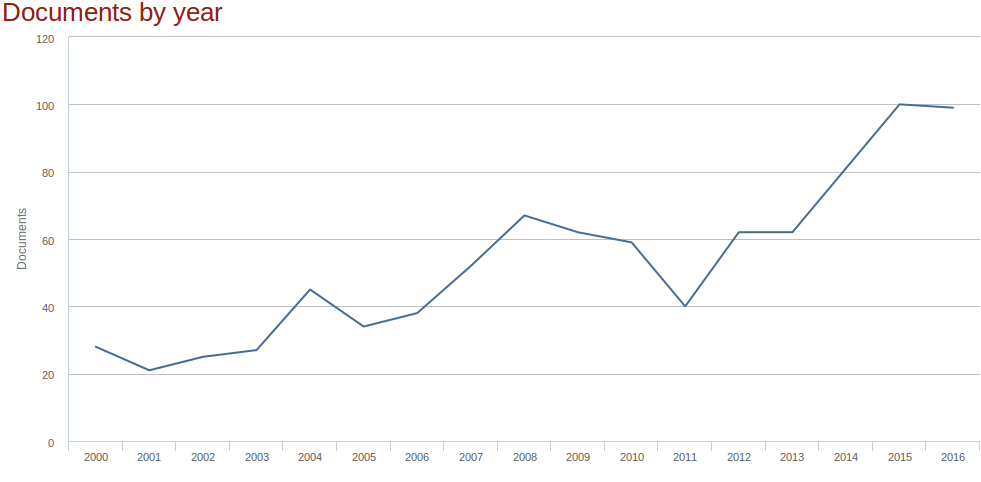
\includegraphics[height=7cm,keepaspectratio=true,clip=true]{imagenes/Logos/scopus.png}
  \caption{Extraído de Scopus.com}
	\label{Fig: scopus1}
\end{figure}



\section{Metodología}\label{sec:metodologia}
En esta sección se detallan los diferentes procesos en el desarrollo del software que se llevaron a cabo para la realización de la tesis, es decir cuales fueron las diversas etapas que se debió realizar y cual fue su organización.

Una metodología en el desarrollo se refiere al entorno que se usa para estructurar, planificar y controlar el proceso de desarrollo de un sistema de información. Este proceso es un conjunto de actividades que conducen a la creación de un producto \citep{sommerville}.


El modelo utilizado para el desarrollo de esta tesis está en función de los objetivos planteados en la sección (Sec: \ref{sec:obj_general}). La misma se dividió en diferentes fases, siguiendo un modelo de desarrollo incremental e iterativo.

En los siguiente ítems se describirán las diferentes fases que se llevo a cabo para alcanzar el objetivo planteado en el desarrollo de la tesis:
\begin{itemize}
	\item \textbf{Fase 1: Investigación de la temática de estudio}\\
	En esta fase se realizó la búsqueda bibliográfica relacionada a la temática de estudio (visión artificial, detección de objeto, 
	Aprendizaje Profundo, Aprendizaje Automático, imágenes satelitales, librerías de desarrollo, métodos de clasificación y regresión).
	\item \textbf{Fase 2: Preparación e Instalación de entorno de Desarrollo.}\\
	En esta fase se realizó la instalación de las herramientas y librerías necesarias para el desarrollo del software; se instalaron librerías  
como(Keras, SkLearn, Python-libs, entre otras).
	\item \textbf{Fase 3: Análisis e Diseño del Software.}\\
	Se analizaron diferentes técnicas de \ac{cv} y \ac{ml} para ser implementadas. En esta fase también se recopilo los \textit{datasets} (conjunto de datos) para el desarrollo.
	\item \textbf{Fase 4: Desarrollo y Evaluación de resultados.}\\
	En esta fase se realizo la evaluación experimental de los datos obtenidos, optimizando los diferentes parámetros para la obtención de un 
modelo mas eficiente.
	\item \textbf{Fase 5: Escritura de Informe y Conclusiones.}\\
	Para finalizar se realizó la escritura de la tesis además se elevaron las conclusiones del desarrollo, evaluando lineas futuras de trabajo.
\end{itemize}


\subsection{Contexto del Sistema}\label{sub:casodeuso}

En la siguiente figura (ver: \ref{Fig: diagbloque}), se muestra el diagrama de bloque del sistema, donde observamos la arquitectura general del software. 

\begin{figure}[H]
 \centering
  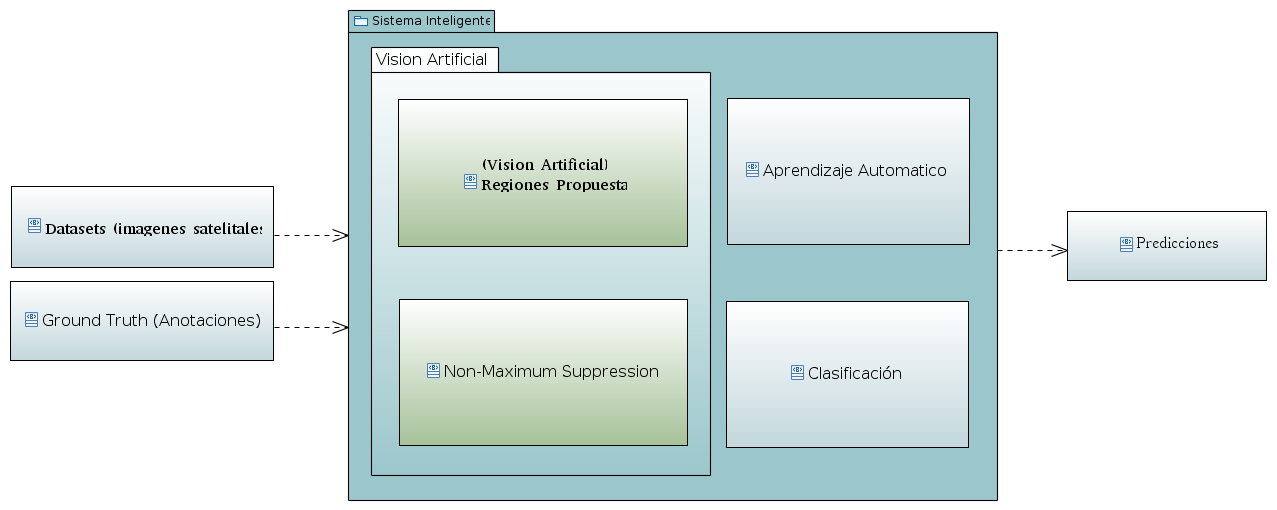
\includegraphics[height=7cm,keepaspectratio=true,clip=true]{imagenes/Logos/diagramabloque.png}
  \caption{Arquitectura del Software de reconocimiento}
	\label{Fig: diagbloque}
 \end{figure}


\section{Estructura General de la Tesis }\label{sec:estructura}

\textcolor{red}{ESTO CAMBIAR CUANDO TERMINE LA TESIS}

La tesis se estructura de acuerdo a los siguientes capítulos: Introducción, Marco Teórico, Desarrollo del Software, Evaluación experimental , Conclusiones y trabajos a futuro, Bibliografía y Apéndice :

En el \textbf{Capítulo} \ref{chap:marcoteorico} \textit{Marco Teórico}: plantea los fundamentos e investigación que se realizaron con el fin de situar el problema dentro de limites teóricos. En este capitulo se desarrolla los conceptos claves como: ¿que es visión artificial?, los métodos que existen, diferentes algoritmos de detección que encontramos en la literatura, ¿ que entendemos por aprendizaje automático?, los campos que hacen uso de esta metodología, nombrando la importancia de las redes neuronales en el campo de reconocimiento de patrones.

El \textbf{Capítulo} \ref{chap:TBD} \textit{TBD}: En este capítulo se describen el esquema de procesamiento (pipeline) utilizado para el desarrollo de la tesis.


El \textbf{Capítulo} \ref{chap:recoleccion} \textit{Recolección de Datos}: En este capitulo se detallan como se obtuvieron los datos para el trabajo.

El \textbf{Capítulo} \ref{chap:Desarrollo} \textit{Desarrollo del Software}: En este capítulo se evalúan las diferentes herramientas utilizadas, junto con la estructura del código realizado.

El \textbf{Capítulo} \ref{chap:evaluacion} \textit{Evaluación Experimental}:  se  dividió en tres secciones principales. La primera hace referencia al los datos y procesos que se llevaron a cabo sobre las imágenes. La segunda parte se describe como se extrajo los datos de cada imagen para realizar el entrenamiento. En la sección final del capitulo se describen los métodos de validación utilizados y cuales fueron los resultados obtenidos.

En el \textbf{Capítulo} \ref{chap:conclusiones} \textit{Conclusiones y Trabajo a Futuro}: se plantea las conclusiones sacadas de la investigación y experimentación además de los posibles trabajo a futuro partiendo de lo realizado.

\textbf{Capítulo} \textit{Bibliografía}: Se enuncian las diferentes fuentes consultadas para el desarrollo de la tesis.

Para finalizar tenemos el \textit{Capítulo \ref{chap:anexo} Apéndice}: describe algunos procesos realizados para el desarrollo de la tesis como por ejemplo, la instalación de librerías usadas, códigos utilizados y diagramas.
